\section{Results}

\subsection{Datasets}

%\placelogofalse
\begin{frame}{Wikipedia-12M}
\begin{columns}
\column{0.58\linewidth}
\centering
\begin{outline}
  \1 public dataset and workload trace
\end{outline}

\column{0.38\linewidth}
\begin{center}
\centering
%\shadowimage[width=2.5cm]{example_1.png}

%\includegraphics[width=2.5cm]{example_3.png}
\end{center}
\end{columns}
\end{frame}
%\placelogotrue

%\placelogofalse
\begin{frame}{Wikipedia-12M: Ablation Study}
\begin{columns}
\column{0.48\linewidth}
\centering
\begin{outline}
  \1 APS
  \2 Little impact on latency
  \2 Big impact on Recall
  \1 NUMA Parallelism
  \2 6x speedup
  \1 Maintenence
  \2 Big impact on latency
  \2 Match results from Faiss-IVF
\end{outline}

\column{0.48\linewidth}
\begin{center}
\centering
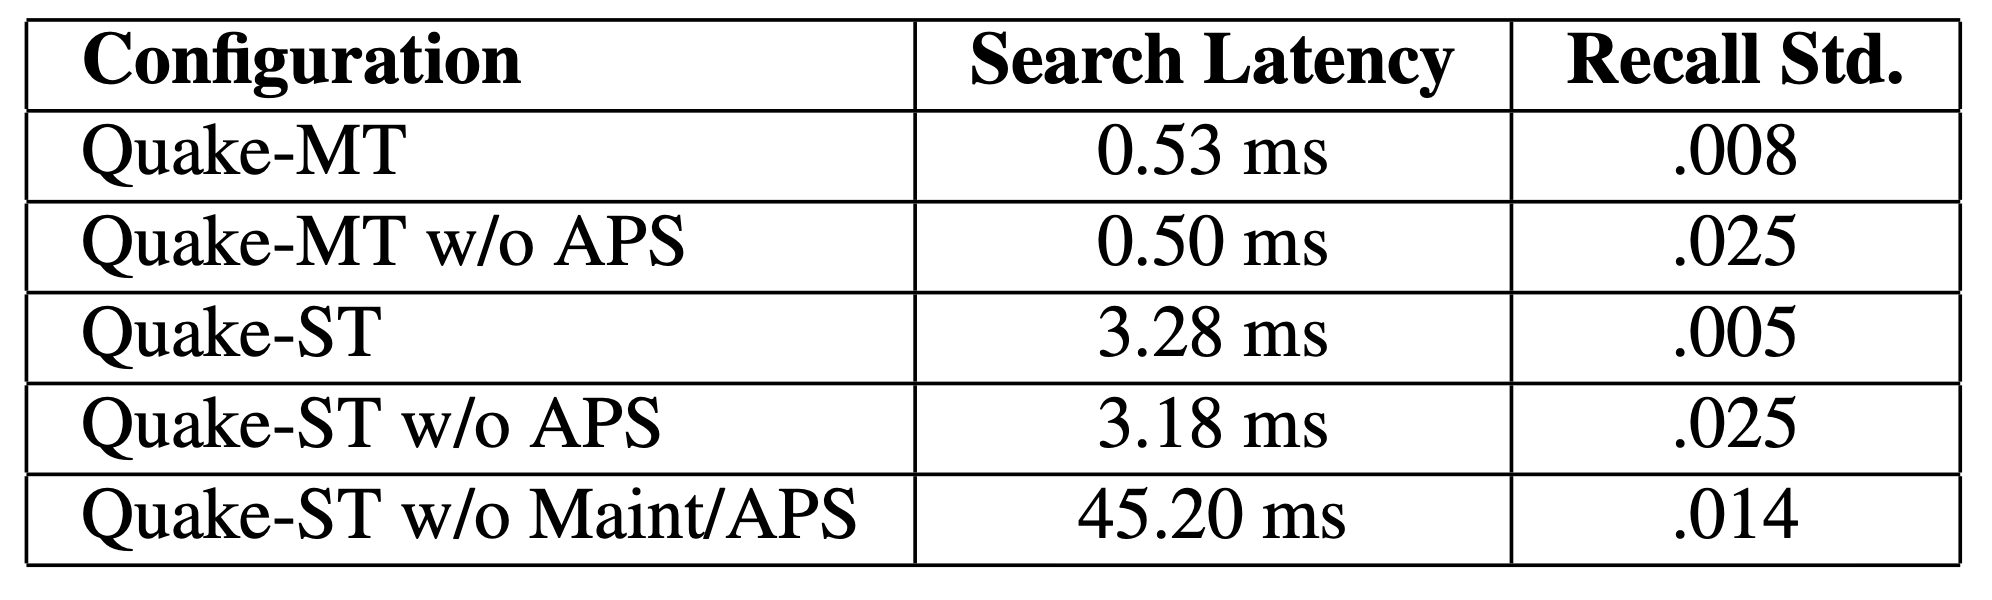
\includegraphics[width=5.5cm]{assets/wiki_ablation.png}
\end{center}
\end{columns}
\end{frame}
%\placelogotrue

%\placelogofalse
\begin{frame}{Other Datasets}
\begin{columns}
\column{0.58\linewidth}
\centering
\begin{outline}
  \1 OpenImages-13M
  \1 MSTuring (10M vector subset)
\end{outline}

\column{0.38\linewidth}
\begin{center}
\centering
%\shadowimage[width=2.5cm]{example_1.png}

%\includegraphics[width=2.5cm]{example_3.png}
\end{center}
\end{columns}
\end{frame}
%\placelogotrue
